\section{Transfer matrix model}
The transfer matrix model is used for simulating external light incident on the device. It assumes light hits the device normal to the surface and the light has reached steady state. This method is good for understanding optical absorption, reflection and transition in structures such as solar cells, optical filters or sensors.  In general any structure where the structure can generally be described as 1D. There are other methods which can be used for this such as FDTD, however general speaking the transfer matrix model will be orders of magnitude faster.

\subsection{The user interface}
This simulation can be reached from the file ribbon and selection "Optical simulation".  If you click "Run optical simulation" (see \ref{fig:transfermatrix0}) the distribution of light within the structure will be calculated as a function of position and wavelength. You can see from the top of the figure that there are various simulation modes. The full transfer matrix method is selected by selecting "Transfer matrix", this will do full optical simulation.  There are also other simplified simulation modes which allow the user to explore more simple charge carrier generation profiles and answer "what if" questions.

\begin{itemize}
  \item Transfer matrix: This is a full transfer matrix simulation which takes into account multiple reflections from the interfaces and optical loss within the structure. This is in effect solving the wave equation in 1D and is an accurate (and recommended) optical model to use.

  \item Exponential profile: This is a very simple optical model which assumes light decays exponentially according to the relation
\begin{equation}
I=I_{0}e^{-\alpha x}
\label{efield2}
\end{equation}
between layers and and assumes light is transmitted between layers according to the formula:
\begin{equation}
T=1.0-\frac{n_1-n_0}{n_1+n_0}
\label{equ:transfermatrixreflection}
\end{equation}
  \item Flat profile: The flat profile assumes light is constant within layers and only decreases at material interfaces according to equation \ref{equ:transfermatrixreflection}.

  \item From file: This can be used to import generation profiles from a file. It us generally used to import the results of more complex optical simulations such as those from external FDTD solvers.
  \item Constant value: If you click on the arrow to the right of the simulation button you will be able to set the charge carrier generation rate within each layer by hand.
\end{itemize}

\begin{figure}[H]
\centering
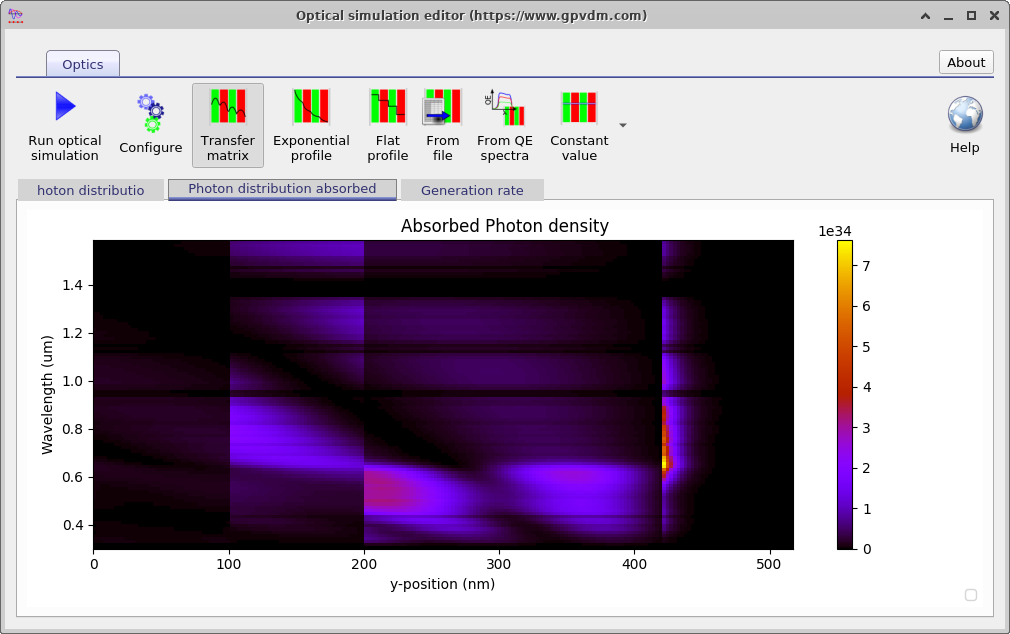
\includegraphics[width=1.0\textwidth,height=0.6\textwidth]{./images/opticalsimulation4.png}
\caption{The output tab this is just like windows file explorer, you can explore the simulation directory tree.}
\label{fig:transfermatrix0}
\end{figure}

The optical simulation window has various tabs which can be used to explore how light interacts with the device. These can be seen in figure \ref{fig:transfermatrix1}. The the top left hand image shows the photon density within the device, the image on the right shows the \emph{total} photon density within the layers of the device.  Notice how the reflection of the light of various layers causes interfearance patterns.  Bottom left shows the configuration of the optical model, you can set here things like the number of wavelengths which are simulated or the number of x-points which are used to describe the device in position space. Bottom right shows the same figure as in the top right of the figure, except by right clicking and playing with the menu options the figure has been converted into band diagram.  This can be useful for generating band diagram figures for papers.
  
\begin{figure}[H]
\centering
\begin{tabular}{ c c }

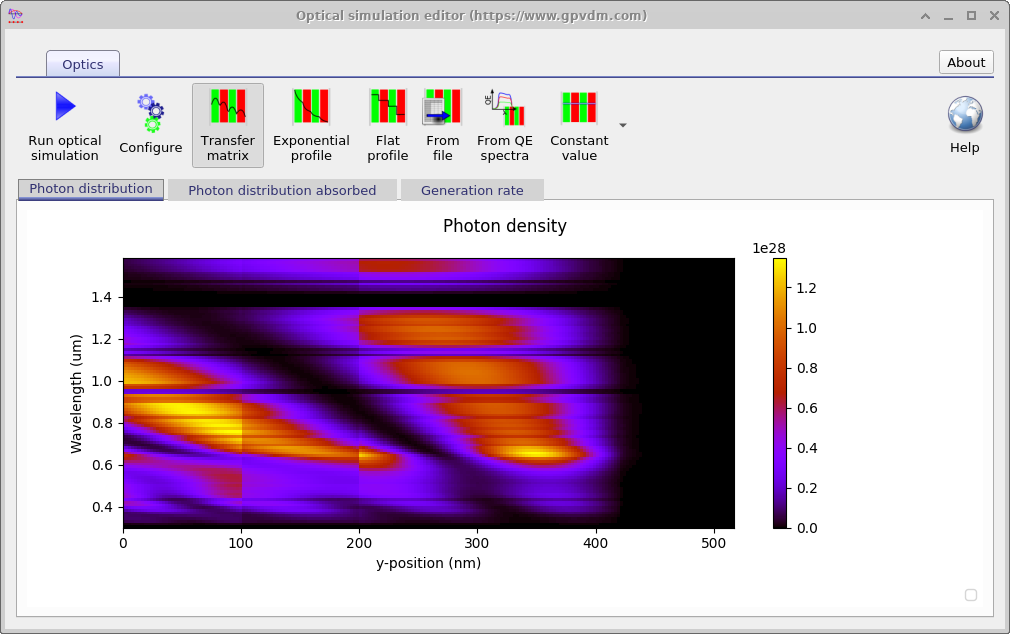
\includegraphics[width=0.5\textwidth,height=0.4\textwidth]{./images/opticalsimulation.png}

&
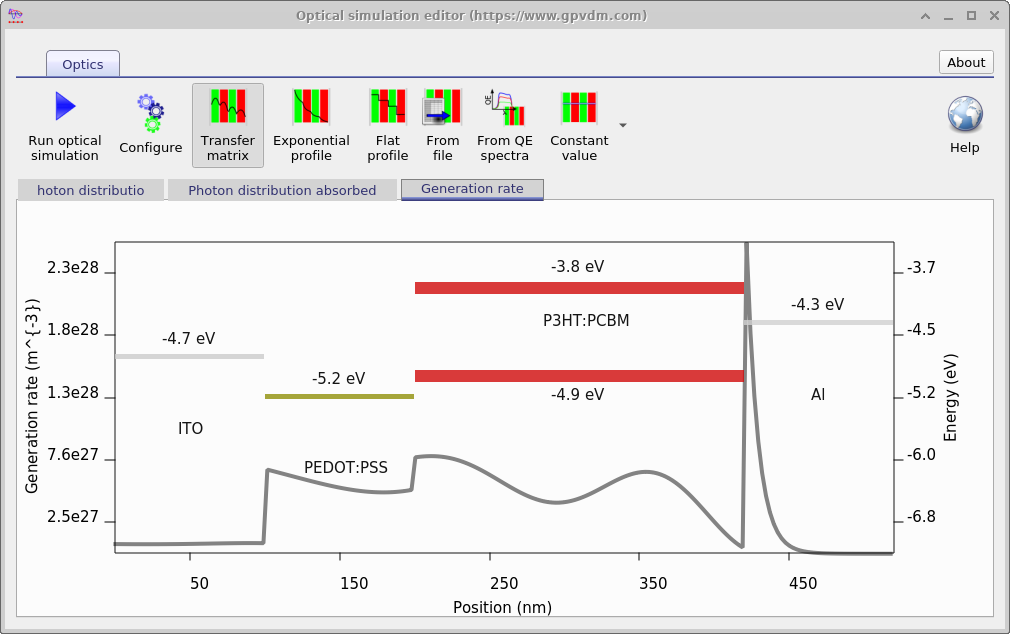
\includegraphics[width=0.5\textwidth,height=0.4\textwidth]{./images/opticalsimulation1.png}

\\
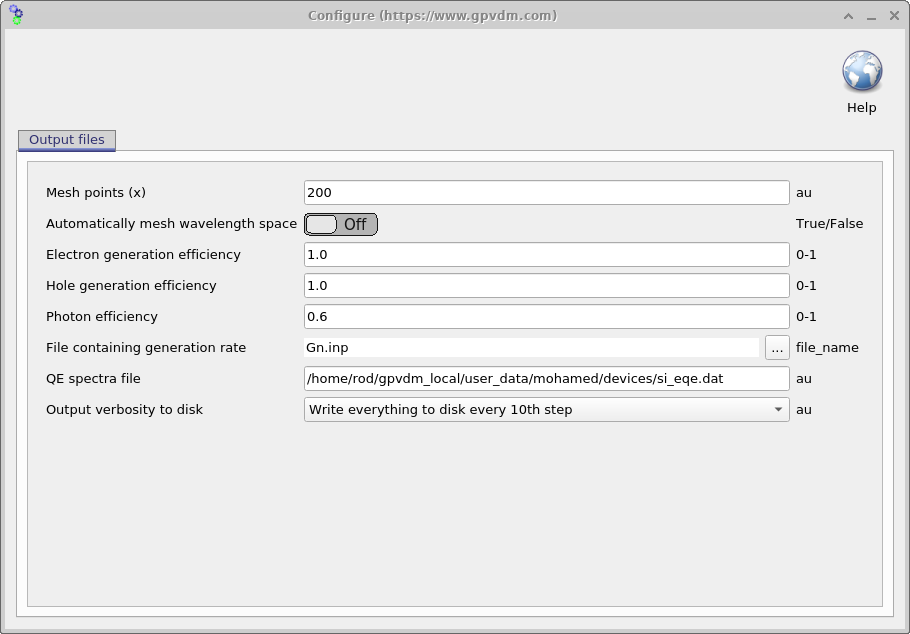
\includegraphics[width=0.5\textwidth,height=0.4\textwidth]{./images/opticalsimulation2.png}

&
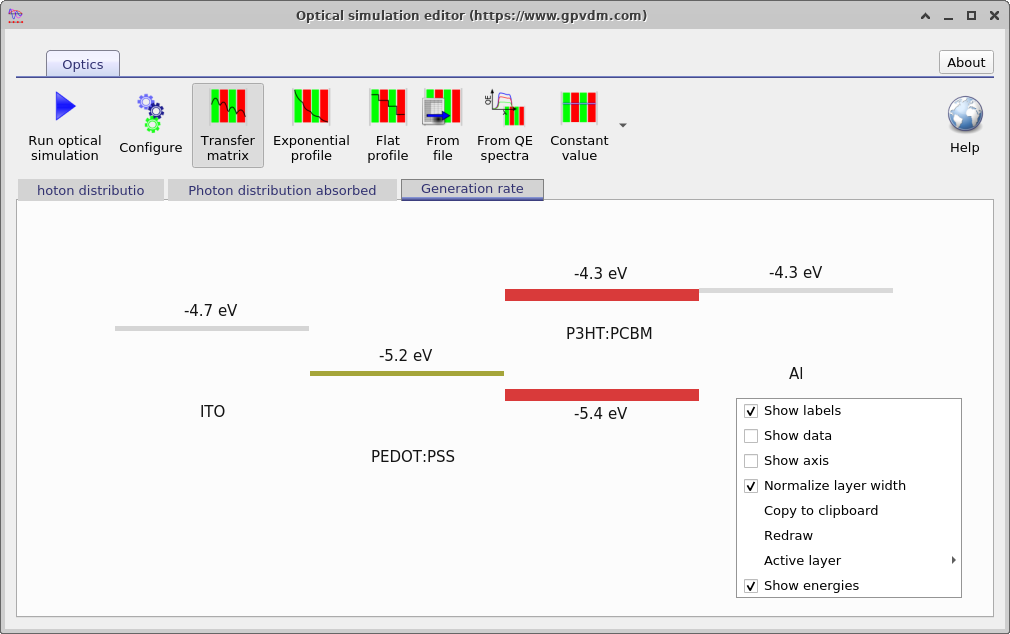
\includegraphics[width=0.5\textwidth,height=0.4\textwidth]{./images/opticalsimulation3.png}

\\
\end{tabular}
\caption{Various views of the optical simulation window}
\label{fig:transfermatrix1}
\end{figure}



\subsection{Theory of the transfer matrix method}
On the left of the interface the electric field is given by

\begin{equation}
E_{1}=E^{+}_{1} e^{-j k_1 z}+E^{-}_{1} e^{j k_1 z}
\label{efield1}
\end{equation}
and on the right hand side of the interface the electric field is given by
\begin{equation}
E_{2}=E^{+}_{2} e^{-j k_2 z}+E^{-}_{2} e^{j k_2 z}
\label{efield2}
\end{equation}

Maxwel's equations give us the relationship between the electric and magnetic fields for a plane wave.

\begin{equation}
\nabla \times E=-j\omega \mu H 
\end{equation}
which simplifies to:
\begin{equation}
\frac{\partial E} {\partial z}=-j\omega \mu H 
\label{maxwel}
\end{equation}

Applying equation \ref{maxwel} to equations \ref{efield1}-\ref{efield2}, we can get the magnetic field on the left of the interface
\begin{equation}
-j \mu \omega H^{y}_{1}=-j k_1 E^{+}_{1} e^{-j k_1 z}+j k_1 E^{-}_{1} e^{j k_1 z}
\end{equation}
and on the right of the interface
\begin{equation}
-j \mu \omega H^{y}_{2}=-j k_2 E^{+}_{2} e^{-j k_2 z}+j k_2 E^{-}_{2} e^{j k_2 z}.
\end{equation}

Tidying up gives,
\begin{equation}
H^{y}_{1}=\frac{k}{\omega \mu}E^{+}_{1} e^{-j k_1 z}-\frac{k}{\omega \mu} E^{-}_{1} e^{j k_1 z}
\end{equation}

\begin{equation}
H^{y}_{2}=\frac{k}{\omega \mu}E^{+}_{2} e^{-j k_2 z}-\frac{k}{\omega \mu} E^{-}_{2} e^{j k_2 z}
\end{equation}


\subsection{Refractive index and absorption}
\begin{equation}
E(z,t)=Re(E_0 e^{j(-kz+\omega t)})= Re(E_0 e^{j(\frac{-2 \pi (n+j\kappa)}{\lambda}z + \omega t)})=e^{\frac{2\pi\kappa z}{\lambda}}Re(E_0 e^{\frac{j(-2 \pi (n+j\kappa)}{\lambda}z +\omega t})
\end{equation}
And because the intensity is proportional to the square of the electric field the absorption coefficient becomes

\begin{equation}
e^{-\alpha x}=e^{\frac{2\pi\kappa z}{\lambda}}
\end{equation}

\begin{equation}
\alpha=-\frac{4\pi\kappa}{\lambda_0}
\end{equation}


\newpage
\vfill

